\documentclass[a4paper, 11pt]{article}

% packages
\usepackage{fontspec}
\usepackage{textcomp}
% syntax highlighting
\usepackage{minted}
% Auflistungen
\usepackage[ampersand]{easylist}
% Verbesserungen zum Style
\usepackage{amsmath, amssymb, amsthm}
% Frage Antwort
\usepackage{dramatist}
% hyperlinks
\usepackage{hyperref}
% Table Formatierung
\usepackage{array}
\usepackage{tabularx}
\usepackage{booktabs}
\usepackage{longtable}
\usepackage{graphicx}
% Sprachunterstützung
\usepackage[nswissgerman]{babel}
% hier setzen wir die Font welche bei den Codeauflistungen verwendet werden soll
\setmonofont[
  Contextuals={Alternate}
]{Fira Code}
\usepackage{lmodern}
% header und footer
\usepackage{fancyhdr}
% hier definieren wir unseren eigenen header/footer style
\lhead{}
\chead{}
\rhead{}
\lfoot{}
\cfoot{\thepage}
\rfoot{}

% Setzt die default Formatierung für die Javasprache
\setminted[java]{
frame=leftline,
framesep=8mm,
numbersep=12pt,
numbersep=5pt,
fontsize=\small,
baselinestretch=1.5,
tabsize=4,
gobble=0,
linenos
}

% lange Wörter auseinander brechen
\hyphenation{
	datenbank-gestützten
	Schreib-waren-handlung
}
% dokument informationen/title
\title{Dokumentation Projektarbeit `HappyWriter'}
\author{Marco Selenati\\
	IFZ--624--002\\
	Stiftung Wirtschaftsinformatikschule Schweiz,\\
	Hohlstrasse 535,\\
	Zürich,\\
	Schweiz\\
	marcoselenati@gmail.com}
\date{\today}

\begin{document}
% Titelseite
\maketitle
\clearpage

% Inhaltsverzeichnis
\pagenumbering{roman}
\tableofcontents
% nichts anderes sollte auf der Inhaltsseite sein
% darum beenden wir hier die Seite
\clearpage
% Anfang Inhalt
\pagenumbering{arabic}
\pagestyle{fancy}

\begin{abstract}

	Erstellung eines datenbankgestützten Online-Shops für eine Schreibwarenhandlung, mit einem Verwaltungssystem für Inhaltsartikel.
	Der Autor erhofft sich dadurch eine gute Dokumentation zu erstellen für zukünftige Klassen welche ein solches Projekt erstellen müssen.

\end{abstract}

\section{Einleitung}

Bei diesem Projekt geht es darum, für den Schreibwarenhandel `HappyWriter' einen datenbankgestützten Online-Shop zu erstellen.
Ich bin Marco Selenati, besuche das 4 Semester der Wirtschaftsinformatikschule Zürich und bin einziger Projektteilnehmer.
Diese Projektbeschreibung wird Ihnen aufzeigen wie ich diesen Webshop erstellt habe.

\section{Problemstellung}

Ziel dieses Projektes ist es, innerhalb einer Woche dem Unternehmen einen funktionierenden Webshop zu Verfügung zu stellen.
In diesem ist auch ein System für das Verwalten von Inhaltsartikeln inbegriffen.
Dieser Webshop eröffnet dem Unternehmen einen neuen Verkaufskanal.

\section{Anforderungen}

Die Projektanforderungen, welche aus den Aufgabeblätter\cite{Aufgabenblaetter} sind, sind wie folgt.

\begin{easylist}[itemize]
	& Project Wonder
	& SQL Skript einrichtung der DB
	& Dokumentation als PDF
	&& Betriebshandbuch
	&& Hilfestellungen
	& Ein in Eclipse importierbares Projekt
	& Das vorgegebene ERD benutzen
	& An jeder Stelle des Vorganges soll ein Abbruch möglich sein
\end{easylist}

\begin{figure}
\caption{Das vorgegebene ERD.}
\centering
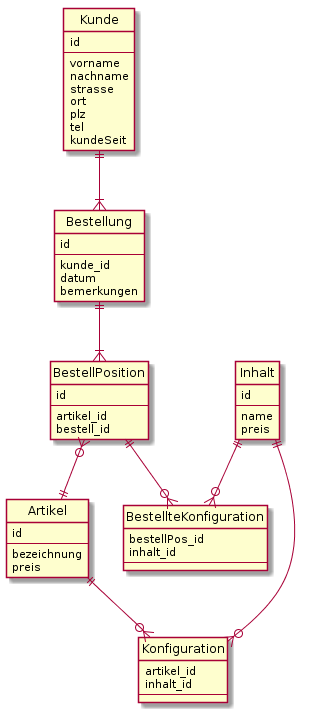
\includegraphics[height=20cm]{erd.png}
\end{figure}
\clearpage

\section{Projektdurchführung}

\subsection{Planung}

Mein Plan, was ich in welcher Reihenfolge machen will.

\begin{easylist}
	& Erstellen des Konzeptes
	&& Klassen
	&& Administrationsbereich
	&& Tests

	& Projektumgebung herstellen
	&& Erstellen des git Repository

	& Erstellen des EOModels
	&& Nach gegebenen ERD
	&& SQL kommentieren
	&& Seed (Test) Daten

	& Funktionalitäten erstellen
	&& Der Normalbenutzer Seiten
	&& Der Administrations Seiten

	& Seite testen
	& Die Seiten Stylen
	& Form Validierung
	& Seite testen
	& Projekt Dokumentation schreiben

\end{easylist}

\subsection{Probleme}

Ich hatte Probleme, welche interessant waren und stelle Ihnen ein paar davon vor.

\subsubsection{Checkbox array}

\paragraph{Problem beschreibung}

Ich wusste nicht, wie ich ein Dynamisches Checkbox array erstellen kann.

\paragraph{Lösungsweg}

Herr Standhart hat mich darauf hingewiesen, dass es ein CheckboxMatrix gibt.
Ich habe danach probiert dieses auf meiner Seite einzusetzen.
Dabei war alles klar ausser selections. Ich dachte, dieses Attribut sei ein Array aus Booleans welches mir sagt, welche Objekte selektiert worden waren, war es aber nicht.
Ich habe nachher in der WOnder Dokumentation nachgelesen, dass es ein Array mit den ausgewählten Objekten zurückgibt.
Als ich es dann ausprobierte, funktionierte es.

\subsubsection{Validation}

\paragraph{Problem beschreibung}

Der Benutzer kann aus Versehen ungültige Daten eingeben und der Server zeigt einen Error an.

\paragraph{Lösungsweg}

Ich habe Parsley und HTML5 input attribute benutzt.
Nach einigem Testen konnte ich keine Error mehr hervorrufen.
Natürlich ist dies kein Schutz vor böswilligen Angriffen, da diese die Validierung umgehen können.
Diese werden dann einen Error von WOnder sehen, aber WOnder speichert keine invaliden Daten in die Datenbank.

\subsubsection{Component Component variablen}

\paragraph{Problem beschreibung}

Ich wollte ein ComponentComponent erstellen welcher die Grundstruktur der HTML Seite beinhaltet.
Für den Body kann ich ComponentContent verwenden, jedoch wie kann ich den Titel variabel halten?

\paragraph{Lösungsweg}

Ich habe zuerst den Titel einfach in die Session gespeichert.
Dann habe ich gemerkt, wenn ich den Titel in einer Seite nicht setze, wird derjenige genommen, welcher auf der letzten Seite gesetzt worden war, da dieser immer noch in der Session ist.
Ich dachte, dass es eine bessere Lösung geben muss. So lass ich im Buch\cite{Learning_the_Wonders}.
Da steht auf Seite 131, dass ich einfach ein Attribut bei dem ComponentComponent machen und dieses verwenden kann.

\subsubsection{Formular abbruch}

\paragraph{Problem beschreibung}

Wenn ich abbrach, die User Daten einzufüllen und sie nachher eingefüllt und abgeschickt hatte, gab es einen Error.

\paragraph{Lösungsweg}

Dieser Error kommt, weil ich probiere, invalide Daten einzugeben.
Die Daten, die ich vom User eintragen will, sind gültig.
Ich werde Ihnen dieses Problem anhand der Checkout Klasse aufzeigen, da dieses gleiche Problem in beiden Klassen aufgetreten ist.
Hier ist der Startzustand, welcher dieses Problem hatte.

\begin{minted}{java}
public class Session extends ERXSession {
	private Kunde kunde = null;
	private Bestellung bestellung;

	/** getter/setter **/

}

public class PCheckOut extends BaseComponent {
	public PCheckOut(WOContext context) {
		super(context);
		 // check ob wir schon kunden und 
		 // bestellungs objekte erstellt haben
		if(session().getKunde() == null) {
			kunde = 
			ERXEOControlUtilities.createAndInsertObject(
				session().defaultEditingContext(),
				Kunde.class);
			bestellung = 
			ERXEOControlUtilities.createAndInsertObject(
				session().defaultEditingContext(),
				Bestellung.class);
		} else {
			kunde = session().getKunde();
			bestellung = session().getBestellung();
		}
	}

	public final WOComponent submit() {
		kunde.setKundeSeit(new NSTimestamp());
		bestellung.setDatum(new NSTimestamp());
		// speichere die finalen kunden
		// und bestellungs daten
		bestellung.setKundenRelationship(kunde);
		// session kunde/ bestellung setzen
		// falls der kunde etwas falsch eingegeben 
		// hat nehmen wir die aus der session
		session().setKunde(kunde);
		session().setBestellung(bestellung);
		return pageWithName(PKontrolle.class);
	}

	public final WOComponent back() {
		return pageWithName(Main.class);
	}

	/** getter/setter **/

}
\end{minted}

Die Daten, welche beim ersten Mal erstellt wurden, sind eingetragen worden.
Da diese noch inkomplett waren, gab es den Error.
Ich musste also die User Daten bei einem Abbruch löschen.

\begin{minted}{java}
public class Session extends ERXSession {
	/** getter/setter **/

}

public class PCheckOut extends BaseComponent {
	public PCheckOut(WOContext context) {
		super(context);
		// check ob wir schon kunden und 
		// bestellungs objekte erstellt haben
		kunde =
		ERXEOControlUtilities.createAndInsertObject(
			session().defaultEditingContext(), 
			Kunde.class);
		bestellung = 
		ERXEOControlUtilities.createAndInsertObject(
			session().defaultEditingContext(), 
			Bestellung.class);
	}

	public final WOComponent submit() {
		PKontrolle kontrolle = pageWithName(PKontrolle.class);
		// speichere die finalen kunden
		// und bestellungs daten
		bestellung.setKundenRelationship(kunde);
		// session kunde/ bestellung setzen
		// falls der kunde etwas falsch eingegeben 
		// hat nehmen wir die aus der session
		kontrolle.setKunde(kunde);
		kontrolle.setBestellung(bestellung);
		return kontrolle;
	}

	public final WOComponent back() {
		kunde.delete();
		bestellung.delete();
		return pageWithName(Main.class);
	}

	/** getter/setter **/

}
\end{minted}

\section{Projektergebnisse}

\subsection{Testkonzept}

\subsubsection{Testumgebung}

\begin{minted}{text}
Windows 10 64bit
Eclipse
    WOLips
Java JDK 8
MariaDB 10
\end{minted}

\subsubsection{Manuelle Tests}

\paragraph{Webseite ist Erreichbar}

Ich verbinde mich zu der URL auf welcher die Applikation laufen sollte

\subparagraph{Erfolg}

Die Applikation läuft und ich kann zu ihr verbinden

\subparagraph{Scheitern}

Die Applikation ist nicht erreichbar oder gibt einen Error aus

\paragraph{Richtige Einstiegsseite}

\subparagraph{Ausführen}

\begin{minted}{text}
Ich verbinde mich zu der URL auf welcher sich die Applikation befindet
\end{minted}

\subparagraph{Erfolg}

Es erscheint die Einstiegsseite

\subparagraph{Scheitern}

Es erscheint eine falsche Seite

\paragraph{Hinzufügen von Artikeln}

\subparagraph{Ausführen}

\begin{minted}{text}
Ich gehe auf die Einstiegsseite und wähle das Etui aus.
Ich werde weitergeleitet auf die Artikelseite.
Ich drücke auf Etui kaufen.
Ich werde zur Einstiegsseite weitergeleitet.
\end{minted}

\subparagraph{Erfolg}

Ich habe nun ein Etui in ihrem Warenkorb

\paragraph{Hinzufügen von Artikeln mit Inhalt}

\subparagraph{Ausführen}

\begin{minted}{text}
Ich gehe auf die Einstiegsseite und wähle das Etui aus.
Ich werde weitergeleitet auf die Artikelseite.
Ich checke die Checkbox für Schere.
Ich drücke auf Etui kaufen.
Ich werde zur Einstiegsseite weitergeleitet.
\end{minted}

\subparagraph{Erfolg}

Ich habe nun ein Etui mit Inhalt Schere in Ihrem Warenkorb

\paragraph{Anschauen von Artikeln}

\subparagraph{Vorraussetzung}

Ich habe keine Artikel im Warenkorb

\subparagraph{Ausführen}

\begin{minted}{text}
Ich gehe auf die Einstiegsseite und wähle das Etui aus.
Ich werde weitergeleitet auf die Artikelseite.
Ich betätige den Zurückknopf.
\end{minted}

\subparagraph{Erfolg}

Ich habe keine Artikel im Warenkorb

\paragraph{Admin zurückkehren zu gespeichertem Stand}

\subparagraph{Vorraussetzung}

Ich habe den Inhalt aaa 12.0000 nicht in der Datenbank

\subparagraph{Ausführen}

\begin{minted}{text}
Ich klicke auf das admin login auf der Homepage.
Ich logge mich mit korrekten Daten ein.
Ich klicke auf Neuen Inhalt erstellen.
Ich erstelle den Inhalt aaa 12.0000.
Ich speichere den erstellten Inhalt.
Ich drücke auf letzten gespeicherten Zustand herstellen.
\end{minted}

\subparagraph{Erfolg}

Der soeben erstellte Datensatz ist weg

\paragraph{Admin speichern von Inhalten}

\subparagraph{Vorraussetzung}

Ich habe den Inhalt aaa 12.0000 nicht in der Datenbank

\subparagraph{Ausführen}

\begin{minted}{text}
Ich klicke auf das admin login auf der Homepage.
Ich logge mich mit korrekten Daten ein.
Ich klicke auf Neuen Inhalt erstellen.
Ich erstelle den Inhalt aaa 12.0000.
Ich speichere den erstellten Inhalt.
Ich drücke auf Speichern.
Ich lasse mir den Inhalt der Tabelle Inhalte ausgeben.
\end{minted}

\subparagraph{Erfolg}

Der soeben erstellte Datensatz ist in der Tabelle eingetragen.

\paragraph{Kundendaten Kontrolle zurück und abschicken}

\subparagraph{Vorraussetzung}

\subparagraph{Ausführen}

\begin{minted}{text}
Ich wähle Holzschachtel.
Ich drücke Kaufen.
Ich drücke Check Out.
Ich gebe a a a a a a ein.
Ich drücke Submit.
Ich drücke Zurück.
Ich gebe a a a a a a ein.
Ich drücke Submit.
Ich drücke Bestätigen.
\end{minted}

\subparagraph{Erfolg}

Der soeben erstellte Datensatz ist in der Tabelle eingetragen.


% Die Ordnerstruktur sollte nicht unterbrochen werden,
% da sie sonst schlecht lesbar ist.
\clearpage
\subsection{Ordnerstruktur}

\begin{minted}{text}
/
    Root des Projektes
             git repos
             WOnder Applikation
/doc
    Alle andere Dokumentation
    /javadoc
        generierte JavaDoc
/sql
    Alle SQL Dateien
/WebServerResources
    Das Rootdirectory des Webservers
    /assets
        ressourcen welche für automatisch
        generierten Seiten gebraucht werden
        /Artikel
            Artikel Ressourcen
        /Inhalt
            Inhalt Ressourcen
README(.md, .pdf)
	Hilfestellung
	Betriebshandbuch
builddoc.ps1
	Baut die Markdown Files zum PDF
\end{minted}

\section{Projektbewertung}

\subsection{Schlussfolgerung}

Die Arbeit an diesem Projekt war sehr interessant. Ich konnte erleben, wie einfach WOnder es einem macht, eine Applikation zu bauen. Dies ist aber nur möglich, wenn man objektorientiert denkt und die Möglichkeiten von WOnder kennt.

\subsection{Reflexion}

Ich muss beim nächsten Projekt die Transactions mehr im Kopf haben. Ich habe immer wieder vergessen, dass in der Datenbank erstellte Objekte, auch wenn nicht auf sie referenziert wird, bei dem nächsten saveChanges mit gespeichert werden.

\addcontentsline{toc}{section}{Abbildungsverzeichnis}

\listoffigures

\addcontentsline{toc}{section}{Literatur}
\begin{thebibliography}{9}
\bibitem{Aufgabenblaetter}
Leistungsbeurteilung Projektarbeit
Datenbanken in Web-Auftritt einbinden (151)
Dokumentnachweis: B14-151\_LB-Projektarbeit\_Aufgabenstellung\_18-06\_V004.docx

\bibitem{Learning_the_Wonders}
Learning the Wonders
Markus Ruggiero
rucotec GmbH, Switzerland; 1 edition (September 20, 2013)
ASIN B00FCDHDAA

\end{thebibliography}

\section{Anhang}

\subsection{Benutzte Ressourcen}

Die gegebenen Bilder für die Artikel und die Inhaltsartikel.

\href{https://getbootstrap.com/docs/4.1/getting-started/introduction/}{Bootstrap} 4.1

\href{http://parsleyjs.org/doc/index.html/}{Parsley}

\subsection{Zeiterfassung}

\subsubsection{2 Juli 2018}

\begin{tabular}{llr}
\toprule
Beschreibung & Zeit \\
\midrule
Erteilung der Aufgabe/ Lesen der Aufgabe & 10:30--11:30 \\
Erstellen der Dokumentation & 11:30--12:00 \\
Erstellen des Plans & 13:03--13:30 \\
Nochmals den ganzen Auftrag durchlesen/durchdenken & 13:30--14:00 \\
Testkonzept schreiben & 14:00--15:20 \\
Verbessern Dokumentation & 15:20--15:30 \\
Erstellen des git Repositories & 19:30--19:35 \\
Erstellen einer korrekt generierten Basis  für WOnder & 19:35--19:50 \\
EOModel erstellen & 19:50--20:40 \\
Datenbankanbindung & 21:04--21:20 \\
Datenbank SQL generieren/Seed daten rauslesen und eintragen & 22:00--22:20 \\
User Seiten erstellen (Ohne Funktionalität) & 22:50--23:15 \\
\bottomrule
\end{tabular}

\subsubsection{3 Juli 2018}

\begin{tabular}{llr}
\toprule
Beschreibung & Zeit \\
\midrule
Foreignkeys in SQL script erstellen & 14:40--15:00 \\
 & 15:25--15:35 \\
Assets einfügen, Image Map & 22:04--22:30 \\
\bottomrule
\end{tabular}

\subsubsection{4 Juli 2018}

\begin{tabular}{llr}
\toprule
Beschreibung & Zeit \\
\midrule
checkout/kontroll seiten erstellen & 9:00--10:20 \\
base layout erstellen & 10:30--11:00 \\
Warenkorb implementieren & 11:00--11:26 \\
Warenkorb Artikel löschen & 16:40--17:10 \\
Dynamischer title für die Seiten & 17:20--17:40 \\
Added Admin login page & 18:05--18:35 \\
Admin Inhalt management Seiten & 19:50--20:20 \\
 & 20:55--21:58 \\
\bottomrule
\end{tabular}

\subsubsection{5 Juli 2018}

\begin{tabular}{llr}
\toprule
Beschreibung & Zeit \\
\midrule
Administrator Artikel Konfiguration & 8:10--8:20 \\
 & 8:40--10:00 \\
einrichten/erstellen eines Templates für die Dokumentation & 14:00--18:00 \\
 & 22:00--24:00 \\
\bottomrule
\end{tabular}

\subsubsection{6 Juli 2018}

\begin{tabular}{llr}
\toprule
Beschreibung & Zeit \\
\midrule
testen & 7:00--7:15 \\
Problem gefunden Konzept ändern & 7:15--7:46 \\
Bemerkungen optional machen & 8:10--8:24 \\
Umsetzung des neuen Administrationsbereiches & 8:41--9:05 \\
Design erstellen & 9:10--9:45 \\
Erstellen basis layouts in bootstrap & 9:45--10:13 \\
 & 10:20--10:30 \\
Erstellen der Hauptseite mit style & 10:30--11:35 \\
Erstellen der Artikelseite & 11:35--12:05 \\
Checkout/Kontrolle sites & 12:05--12:17 \\
session terminieren & 12:17--12:20 \\
Erstellen der Admin login in seite & 12:20--12:27 \\
Erstellen des admin bereiches & 13:30--13:36 \\
Admin Artikel Seite stylen & 13:37--14:00 \\
Admin Inhalts Seite stylen & 14:00--14:10 \\
Admin Inhalts Edit/Create Seite stylen & 14:10--14:13 \\
Parsley Validation & 14:13--14:40 \\
Artikel und Inhalte mit icons & 14:40--15:05 \\
Kleine Verbesserungen & 15:05--16:03 \\
Dokumentation schreiben/ Über Dokumentieren lesen & 18:00--24:00 \\
\bottomrule
\end{tabular}

\subsubsection{7 Juli 2018}

\begin{tabular}{llr}
\toprule
Beschreibung & Zeit \\
\midrule
Dokumentation schreiben/ Über Dokumentieren lesen & 00:00--01:00 \\
Arbeiten an der Dokumentation & 10:00--23:25 \\
\bottomrule
\end{tabular}

\subsubsection{8 Juli 2018}

\begin{tabular}{llr}
\toprule
Beschreibung & Zeit \\
\midrule
JavaDoc schreiben & 12:30--13:00 \\
 & 14:00--14:10 \\
 & 14:30--15:00\\
Dokumentation schreiben & 15:55--17:30 \\
 & 17:50--19:10 \\
EOModel Fixen & 19:10--19:55 \\
UX verbessern & 19:55--20:40 \\
Dokumentation verbessern & 21:00--21:57 \\
Dokumentieren & 22:12--22:48 \\
Dokumentation verbessern & 22:48--23:20 \\
\bottomrule
\end{tabular}

\subsubsection{9 Juli 2018}

\begin{tabular}{llr}
\toprule
Beschreibung & Zeit \\
\midrule
Dokumentation verbessern & 8:00--9:05 \\
Error Seite erstellen & 9:05--9:26 \\
Testen & 9:34--11:03 \\
 & 11:03--12:09 \\
 & 12:30--14:30 \\
\bottomrule
\end{tabular}

\subsection{Informationsbeschaffung}

\begin{drama}
	\Character{Marco Selenati}{ms}
	\Character{Markus Ruggiero}{dozent}
	\Character{Internet}{internet}
	\Character{Herr Bärlocher}{lucas}
	\Character{Frau Fusco}{fusco}
	\Character{Herr Standhardt}{standhard}

\msspeaks: Kann ich die Dokumentation, solange sie am Schluss PDF ist, aus allem was ich will generieren lassen?

\dozentspeaks: Ja, Sie können es aus Markdown Word oder sogar aus einem selbst geschriebenen Tool generieren lassen, wenn Sie wollen.

\msspeaks: Auf dem vorgegebenen ERD steht, dass bei der Konfigurationstabelle ein Attribut mit dem Namen inhalt\_d sein soll. Muss ich das genau so machen?

\dozentspeaks: Nein, das sollte inhalt\_id sein. Das muss ein Tippfehler sein.

\msspeaks: Die Bestellübersichtsseite ist nirgends im Text vorhanden. Wo kommt diese hin?

\dozentspeaks: Die Bestellübersichtsseite ist eine bessere Version der Mainseite. Da die Bestellübersichtsseite eine bessere Warenkorbauflistung hat.

\msspeaks: Kann ich die Bilder der Inhalte bei der Auswahl der Inhalte anzeigen?

\dozentspeaks: Wäre gut, wenn es so wäre.

\msspeaks: Muss ich angeben dass ich die gegebenen Bilder benutze?

\dozentspeaks: Ja, in der Dokumentation reicht. Sie können es schon auf der Seite angeben, aber es ist ok, wenn ohne.

\msspeaks: Darf ich die Namen im UML umbenennen?

\dozentspeaks: Ja.

\msspeaks: Darf ich das ganze anders gestalten wie es im UML steht?

\dozentspeaks: Ja, dass UML ist nur ein Vorschlag.

\msspeaks: Wie benutze ich Checkbox matrix

\internetspeaks: \href{https://github.com/wocommunity/wonder/blob/4d7f6bf9236c3005359101d6f3c9e6224d47750e/Frameworks/Core/JavaWOExtensions/Sources/com/webobjects/woextensions/WOCheckboxMatrix.java}{WOnder dokumentation}

\msspeaks: Wie kann ich nur Buchstaben im Namen und Vornamen haben?

\internetspeaks: \href{https://stackoverflow.com/questions/23415795/how-to-only-allow-text-in-parsely-js-validation}{stackoverflow parsley}

\msspeaks: Wissen Sie, wie man CSS einbinden soll?

\lucasspeaks: ERXStyleSheet

\msspeaks: Wissen Sie, wie man JavaScript einbindet?

\lucasspeaks: ERX JavaScript

\msspeaks: Wie kann ich ein Design für das Aussehen der Webseite erstellen?

\lucasspeaks: draw io.

\msspeaks: Können Sie sich meine Applikation ansehen und mir sagen, ob Sie Probleme sehen?

\lucasspeaks:
    Vorname, Nachname sollte nur Buchstaben haben
    Telefon sollte nur Nummern und + () haben

\msspeaks: Wissen Sie, wie ich die Checkboxenwerte in ein Array reinbekomme?

\standhardspeaks: Ich habe einfach Checkbox Matrix benutzt.

\msspeaks: Wollen Sie sich meine Applikation ansehen?

\fuscospeaks: Ja
    Artikel und Inhalt sind verwirrend, da Inhalte auch Artikel sind. Inhaltsartikel anstatt Inhalt.
    Admin Login sollte auf den CMS Seiten nicht angezeigt werden.

\end{drama}

\end{document}
